\documentclass[10pt,onecolumn,conference]{IEEEtran}
\IEEEoverridecommandlockouts
% The preceding line is only needed to identify funding in the first footnote. If that is unneeded, please comment it out.
%\usepackage{cite}
\usepackage{amsmath,amssymb,amsfonts}
%\usepackage{algorithmic}
\usepackage{graphicx}
\usepackage{textcomp}
\usepackage{xcolor}
\def\BibTeX{{\rm B\kern-.05em{\sc i\kern-.025em b}\kern-.08em
    T\kern-.1667em\lower.7ex\hbox{E}\kern-.125emX}}


\usepackage{url}
\usepackage{cite}
\usepackage{amsmath,amssymb,amsfonts}
\usepackage{graphicx}
\usepackage{textcomp}
\usepackage{xcolor}
\usepackage{algorithm,algpseudocode}
\algrenewcommand\algorithmicindent{0.9em}%
\usepackage{soul}
\usepackage{xspace}
\usepackage{subfigure}

\begin{document}




\newcommand{\todo}[1]{\color{red}\textbf{\hl{#1}}\color{black}\xspace}
%\newcommand{\todo}[1]{}
\newcommand{\rom}[1]{\expandafter{\romannumeral #1\relax}}

\section{Intel CPUs}

\subsection{Ice Lake}
Ice Lake is Intel's codename for the 10th generation Intel Core processors based on the new Sunny Cove microarchitecture. 
Ice Lake was expected to replace microprocessors based on the Skylake microarchitecture.


Features:
\begin{enumerate}
\item \textit{Sunny Cove} micro-architecture.
\item increase the execution units(EUs) to 64, from 24 or 48 in Gen 9.5 graphics.
\item Each EU supports 7 threads.
\item 50\% increase in the size of L1, L2 cache, larger $\mu OP$ cache, and larger 2nd level \texttt{TLB}.
\item 3MB L3 cache.
\item 1 TFLOPS of compute performance.
\end{enumerate}


Focus:
Single-thread performance, new instructions(\texttt{VPOPCNTDQ, VBMI2, BITALG, VPCLMULQDQ, GFNI, and VAES}), and scalability.

\paragraph{\texttt{VPOPCNTDQ}}
Count the number of logical 1 bits in packed 32-bit integers in a, and store the results in dst.\\
\textbf{syntax:} \texttt{\_\_m512i \_mm512\_popcnt\_epi32 (\_\_m512i a)}

\paragraph{\texttt{VBMI2}}

\paragraph{\texttt{BITALG}}

\paragraph{\texttt{VPCLMULQDQ}}
Carry-less multiplication of one quadword of 'b' by one quadword of 'c', stores the 128-bit result in 'DEST'. 
The immediate 'Imm8' is used to determine which quadwords of 'b' and 'c' should be used. \\
\textbf{syntax:} \texttt{\_\_m512i \_mm512\_clmulepi64\_epi128 (\_\_m512i b, \_\_m512i c, const int Imm8)}
\paragraph{\texttt{GFNI}}

\paragraph{\texttt{VAES}}
Perform one round of an AES decryption flow on data (state) in a using the round key in RoundKey, and store the results in dst.\\
\textbf{syntax:} \texttt{\_\_m512i \_mm512\_aesdec\_epi128 (\_\_m512i a, \_\_m512i RoundKey)}

\subsection{\texttt{Tiger Lake}}
\texttt{Tiger Lake} is an Intel core processor to replace \texttt{Ice Lake}.

Features:
\begin{enumerate}
\item Intel Willow Cove CPU cores.
\item Intel Xe ("Gen12") GPU with up to 96 execution units.
\item HEVC 12-bit, 4:2:2 \& 4:4:4 fixed-function hardware decoding \& VP9 12-bit \& 4:4:4 fixed-function hardware decoding.
\item PCI Express 4.0.
\item Thunderbolt 4.
\item Miniaturization of CPU and motherboard into an M.2 SSD-sized small circuit board.
\item LPDDR5 memory.
\item New Deep Learning Boost (DL Boost) extensions for built-in AI training acceleration in Xeon processors.
\item A new AVX-512 instruction: Vector Pair Intersection to a Pair of Mask Registers (VP2INTERSECT).
\end{enumerate}

%Xe Graphics 

\begin{figure}[!bth]
\centering
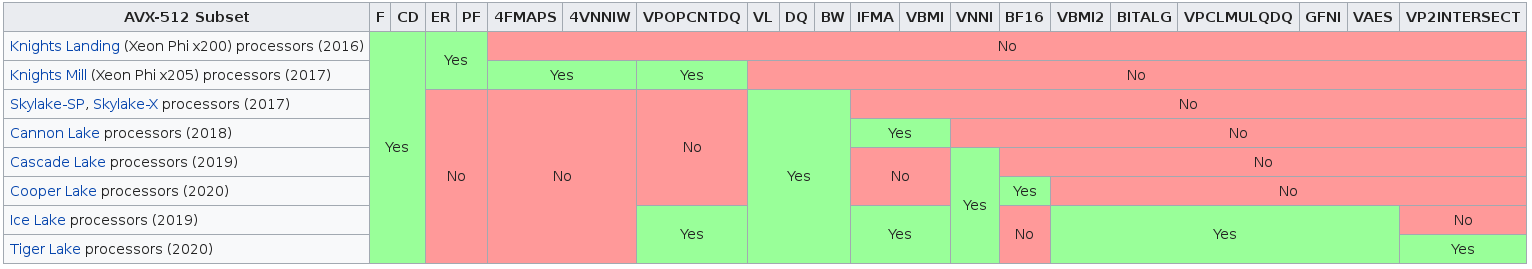
\includegraphics[width=1.0\textwidth]{Figures/avx_instruction.png}
\caption{Avx-512 instruction sets for different Intel core processor[wiki].}
\label{fig:avxinstruction}
\end{figure}

\section{Intel GPU}
Code Name: \texttt{DG1}\\


\section{AMD Processors}

\subsection{Ryzen}


\end{document}